%%%%%%%%%%%%%%%%%%%%%%%%%%%%%%%%%%%%%%%%%
% A beamer poster style for the University of Oxford. Atilim Gunes Baydin <gunes@robots.ox.ac.uk>, November 2016.
% Based on the I6pd2 style created by Thomas Deselaers an Philippe Dreuw.
%
% Dreuw & Deselaer's Poster
% LaTeX Template
% Version 1.0 (11/04/13)
%
% Created by:
% Philippe Dreuw and Thomas Deselaers
% http://www-i6.informatik.rwth-aachen.de/~dreuw/latexbeamerposter.php
%
% This template has been downloaded from:
% http://www.LaTeXTemplates.com
%
% License:
% CC BY-NC-SA 3.0 (http://creativecommons.org/licenses/by-nc-sa/3.0/)
%
%%%%%%%%%%%%%%%%%%%%%%%%%%%%%%%%%%%%%%%%%

%----------------------------------------------------------------------------------------
%   PACKAGES AND OTHER DOCUMENT CONFIGURATIONS
%----------------------------------------------------------------------------------------

\documentclass[final,hyperref={pdfpagelabels=false}]{beamer}

\usepackage[orientation=landscape,size=a0,scale=1.3]{beamerposter} % Use the beamerposter package for laying out the poster with a portrait orientation and an a0 paper size

\usetheme{Oxford}

\usepackage[utf8]{inputenc} % allow utf-8 input
\usepackage{blindtext}
\usepackage{amsmath,amsthm,amssymb,latexsym} % For including math equations, theorems, symbols, etc
\usepackage[document]{ragged2e}
\usepackage{times}\usefonttheme{professionalfonts}  % Uncomment to use Times as the main font
\usefonttheme[onlymath]{serif} % Uncomment to use a Serif font within math environments
%\boldmath % Use bold for everything within the math environment
\usepackage{booktabs} % Top and bottom rules for tables
\usepackage{microtype}
\usepackage{subcaption}
\usepackage{tcolorbox}
\usepackage{multirow}

% custom coloured box
\definecolor{darkgreen}{rgb}{0,.7,0}
\definecolor{darkred}{rgb}{0.54,0,0}
\definecolor{camblue}{rgb}{0.639,0.757,0.678}

\usecaptiontemplate{\small\structure{\insertcaptionname~\insertcaptionnumber: }\insertcaption} % A fix for figure numbering
\setbeamertemplate{caption}[numbered]

\newcommand{\shrink}{-15pt}

\def\imagetop#1{\vtop{\null\hbox{#1}}}

\let\oldbibliography\thebibliography
\renewcommand{\thebibliography}[1]{\oldbibliography{#1}
\setlength{\itemsep}{-10pt}}

%----------------------------------------------------------------------------------------
%   TITLE SECTION 
%----------------------------------------------------------------------------------------
\title{ATML Paper Reproduction Challenge: Gated Graph Sequence Neural Networks~\cite{DBLP:journals/corr/LiTBZ15}} % Poster title
\author{Jad Ghalayini, Albert Qiaochu Jiang, Kamilė Stankevičiūtė}
\institute{Department of Computer Science, University of Oxford\\\vspace{4mm}
\texttt{\{jad.ghalayini,qiaochu.jiang,kamile.stankeviciute\}@cs.ox.ac.uk}}

%----------------------------------------------------------------------------------------
%   FOOTER TEXT
%----------------------------------------------------------------------------------------
\newcommand{\leftfoot}{} % Left footer text
\newcommand{\rightfoot}{} % Right footer text


%----------------------------------------------------------------------------------------

\begin{document}
\addtobeamertemplate{block end}{}{\vspace*{2ex}} % White space under blocks

\begin{frame}[t] % The whole poster is enclosed in one beamer frame

\begin{columns}[t] % The whole poster consists of three major columns, each of which can be subdivided further with another \begin{columns} block - the [t] argument aligns each column's content to the top

  \begin{column}{.02\textwidth}\end{column} % Empty spacer column

%%%%%%%%%%%%%%%%%%%%%%%%%%%%%%%%%%%%%%%%%%
%% Column 1
%%%%%%%%%%%%%%%%%%%%%%%%%%%%%%%%%%%%%%%%%%

  \begin{column}{.3\textwidth} % 1st column
    \vspace{\shrink}          
    \begin{block}{Summary of the paper}
      
      \begin{itemize}
          \item The paper presents \textcolor{darkred}{Gated Graph (Sequence) Neural Networks}, or \textcolor{darkred}{GG(S)NNs}—architectures that leverage the temporal patterns of message passing in graph-structured data to produce \textcolor{darkred}{sequence outputs}.
          \item GG(S)NNs are benchmarked against baseline RNNs on a subset of reasoning tasks in the bAbI dataset and two additional graph algorithm learning tasks, and are applied to a real-world task in the program verification domain.
      \end{itemize}

    \end{block}
    

    % \vspace{-0.6in} 
    % \begin{block}{Recurrent Graph Neural Networks}
    % Node aggregation can be modelled by recurrence.
    
    %   \begin{figure}
    %     \centering
    %     \begin{subfigure}{.25\textwidth}
    %       \centering
    %       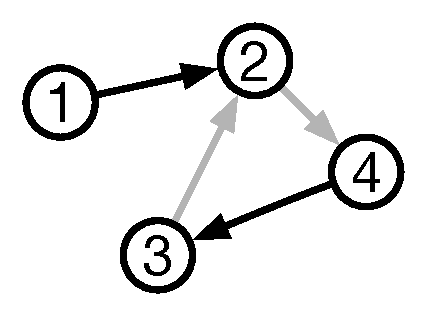
\includegraphics[height=3in]{imgs/example-graph.pdf}
    %       \caption{}
    %       \label{fig:sub1}
    %     \end{subfigure}%
    %     \hfill
    %     \begin{subfigure}{.43\textwidth}
    %       \centering
    %       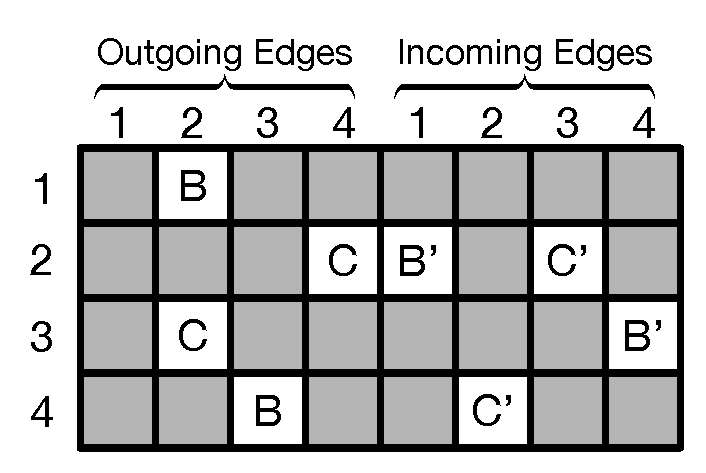
\includegraphics[height=3in]{imgs/recurrent-matrix-sparsity-pattern2.pdf}
    %       \caption{}
    %       \label{fig:sub2}
    %     \end{subfigure}
    %     \begin{subfigure}{.25\textwidth}
    %       \centering
    %       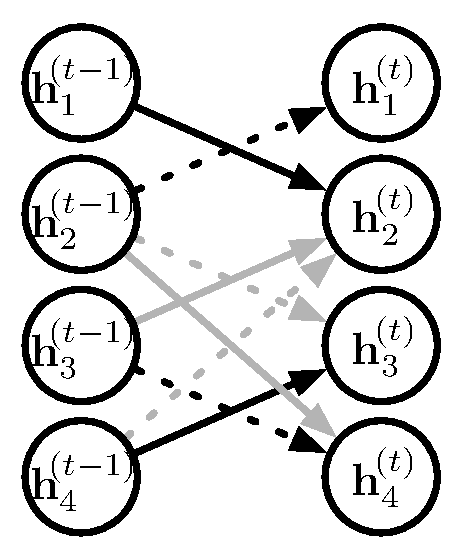
\includegraphics[height=3in]{imgs/unrolled-graph3.pdf}
    %       \caption{}
    %       \label{fig:sub2}
    %     \end{subfigure}
        
    %     \caption{(a) An example of a directed graph. Colour denotes the type of the edge. (b) Adjacency matrix with edge typing. (c) Message passing by unrolling recurrence for one timestep. Dotted lines denote propagation in reverse edge directions. This figure is a re-ordered duplicate of Figure 1 from \cite{DBLP:journals/corr/LiTBZ15}.}
    %     \label{fig:test}
    %   \end{figure}
      
      
    % \end{block}
    
     \vspace{-0.6in} 
    \begin{block}{Gated Graph Neural Networks (GGNNs)}
    Let $\mathcal{G}=(\mathcal{V}, \mathcal{E})$ be a graph where $\mathcal{V}$ is the set of nodes, and $\mathcal{E}$ is the set of edges. Each node $v$ has an annotation $\mathbf{x}_v$, and every edge has a type—for an arbitrary directed edge $u \leadsto v$ of type $A$, there is a directed edge from $v \leadsto u$ of type $A'$. The GGNN is implemented as follows:
    \vspace{0.2in}
    
    \textcolor{darkred}{Initialisation.} The latent representations for graph nodes are initialised by padding the node annotations:
    \begin{equation}
        \forall v \in \mathcal{V}. \, \mathbf{h}_v^{(0)} = [\mathbf{x}_v^\top, \mathbf{0}]^\top.
    \end{equation}
    
    
    \textcolor{darkred}{Message passing.} For an edge $u \leadsto v$ of type $A$, $\mathbf{h}_u^{(t)}$ and $\mathbf{h}_v^{(t)}$ the latent representations for $u$ and $v$ at time $t$, and $\mathbf{A}$ the trainable parameter for the edge type $A$, the from $u$ to $v$ is
    \begin{equation}
        \mathbf{m}_{uv}^{(t)} = \mathbf{A} \mathbf{h}_u^{(t-1)}.
    \end{equation}
    
    \textcolor{darkred}{Propagation.} At each iteration, each node representation is updated by combining messages from its neighbours and the latent representation from the last iteration, where $\mathbf{b}$ is the trainable bias vector:
    \begin{equation}\label{eq:GRU}
        \forall v \in \mathcal{V}. \, \mathbf{h}_v^{(t)} = \mathrm{GRU}\left(\mathbf{h}_v^{(t-1)}, 
        \mathrm{add}(\{\mathbf{m}_{uv}^{(t)} \mid (u, v) \in \mathcal{E} \}) + \mathbf{b}\right).
    \end{equation}

    After $T$ iterations, the final latent representation for node $v$ is $\mathbf{s}_v = \mathbf{h}_v^{(T)}$.
    \textcolor{darkred}{Output modules.} For \textcolor{darkred}{node selection} tasks, we use a scoring function $f_s$ to obtain a categorical distribution over nodes:
        \begin{equation}
            \mathbf{p}_{\mathrm{node}} = \mathrm{softmax}\left(f_s([\mathbf{s}_{v_1}, \mathbf{s}_{v_2}, \ldots, \mathbf{s}_{v_{\mid \mathcal{V}\mid}}]^T)\right).
        \end{equation}
    For \textcolor{darkred}{graph classification} tasks, we first obtain a graph readout:
        \begin{equation}
            \mathbf{h}_{\mathcal{G}} =
                \sum_{v\in\mathcal{V}}  
                \sigma \left(f_1\left([\mathbf{s}_v^\top, \mathbf{x}_v^\top]^\top\right)\right)
                \odot
                \tanh \left(f_2\left([\mathbf{s}_v^\top, \mathbf{x}_v^\top]^\top\right)\right),
        \end{equation}
        where $f_1$ and $f_2$ are neural networks, $\sigma$ is the sigmoid function, and $\odot$ is the element-wise product. A neural network $f_c$ produces a probability distribution over the classification categories:
        \begin{equation}
            \mathbf{p}_{\mathcal{G}} = \mathrm{softmax}\left(f_c\left(\mathbf{h}_{\mathcal{G}}\right)\right).
        \end{equation}
    
    For a fixed number of recurrent unrolling steps, \textcolor{darkred}{the GGNN is entirely differentiable}, and gradients can be calculated back propagation through time, which is a boost to optimisation. This was not the case for previous GNNs relying on contraction maps.

    \end{block}
    
  \end{column} % End of the 1st column

%%%%%%%%%%%%%%%%%%%%%%%%%%%%%%%%%%%%%%%%%%
%% Column 2
%%%%%%%%%%%%%%%%%%%%%%%%%%%%%%%%%%%%%%%%%%

  \begin{column}{.02\textwidth}\end{column} % Empty spacer column

  \begin{column}{.3\textwidth} % 2nd column
    \vspace{\shrink}
    % \vspace{0.1in}
    
    \color{oxfordblue}
    
    
    \begin{block}{Gated Graph Sequence Neural Networks (GGSNNs)}
     GGSNN is an extension of the GGNN architecture that is capable of returning a \textcolor{darkred}{sequence} of outputs. A schematic of the GGSNN architecture is shown in Figure \ref{fig:GGSNN}.

    \begin{figure}
        \centering
        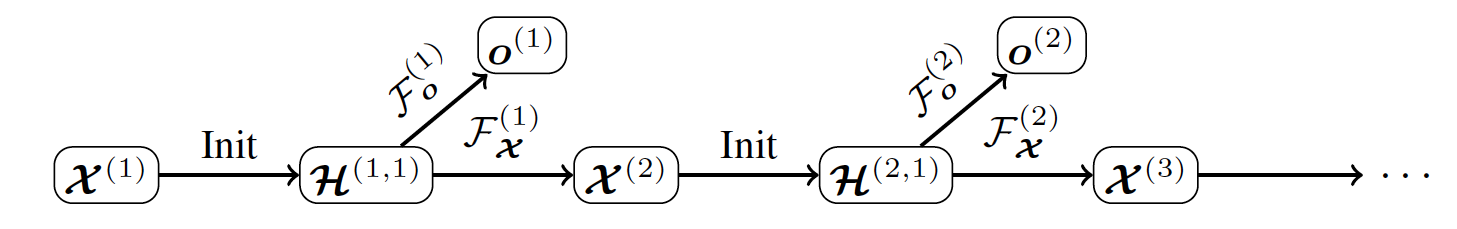
\includegraphics[width=\textwidth]{imgs/ggsnn.png}
        \caption{Diagram of the GGSNN mechanism. Taken from Figure 2 in \cite{DBLP:journals/corr/LiTBZ15}.}
        \label{fig:GGSNN}
    \end{figure}
    In a GGSNN 
    %with shared output and propagation modules 
    producing an output sequence of length $L$, each \textbf{Init} step pads the input annotations $\boldsymbol{\mathcal{X}}^{(l)}$ with 0: $\boldsymbol{\mathcal{H}}^{(l, 1)} = [\boldsymbol{\mathcal{X}}^{(l)}, \boldsymbol{0}]$.
    When the propagation model is shared, the output model $\mathcal{F}_{\mathbf o}^{(l)}$ and propagation model $\mathcal{F}_{\boldsymbol{\mathcal{X}}}^{(l)}$ adopt the same GGNN layer $\mathcal{F}$ but have different output modules:
    
    \begin{equation}
        \mathbf{H}^l = \boldsymbol{\mathcal{F}}\left(\boldsymbol{\mathcal{H}}^{(l, 1)}\right),\, \boldsymbol{o}^{(l)} = 
        \boldsymbol{\mathcal{O}} \left([\mathbf{H}^l, \boldsymbol{\mathcal{X}}^{(1)}]\right),\, 
        \boldsymbol{\mathcal{X}}^{(l+1)} = \boldsymbol{\mathcal{P}}\left([\mathbf{H}^l, \boldsymbol{\mathcal{X}}^{(1)}]\right),
    \end{equation}
    where $\boldsymbol{\mathcal{O}}$ is an output module, and $\boldsymbol{\mathcal{P}}$ is a multi-layer perceptron for propagating information to the next prediction step.
    \end{block}
    \vspace{-0.6in} 
    \begin{block}{Experiments}
      We reproduced the results of GG(S)NNs and the RNN/LSTM baselines on five bAbI tasks~\cite{DBLP:journals/corr/WestonBCM15}: Two argument relations, Basic deduction, Basic induction, Size reasoning, and Path finding (Tasks 4, 15, 16, 18, 19). Tasks are represented in a symbolic form and converted to graphs. The reproduction results are presented in Table \ref{table:table-1}.\vspace{0.1in}
      
      \begin{table}[t]
          \caption{Test accuracies~(in \%) of the models for selected bAbI tasks. Number in parentheses denotes the number of training examples.}\label{table:table-1}
          \vspace{0.1in}
          \centering
          \small
          \begin{tabular}{cccccc}
              \toprule
              bAbI Task & Implementation & RNN & LSTM & GGNN \\  \midrule
              \multirow{2}{*}{4} & Li et al. & $97.3 \pm 1.9\thinspace (250)$ & $97.4 \pm 2.0\thinspace  (250)$ & $\mathbf{100.0 \pm 0.0\thinspace (50)}$ \\
              & ours & $98.9 \pm 1.4\thinspace (250)$ & $96.6 \pm 2.5\thinspace (250)$ & $\mathbf{100.0 \pm 0.0\thinspace (50)}$ \\  \midrule
        
              \multirow{2}{*}{15} & Li et al. &  $48.6 \pm 1.9\thinspace (950)$ & $50.3 \pm 1.3\thinspace (950)$ & $\mathbf{100.0 \pm 0.0\thinspace (50)}$  \\
              & ours & $38.6 \pm 3.7\thinspace (950)$ & $49.9 \pm 0.7\thinspace (950)$ & $\mathbf{100.0 \pm 0.0\thinspace (50)}$ \\  \midrule
        
              \multirow{2}{*}{16} & Li et al. &  $33.0 \pm 1.9\thinspace (950)$&  $37.5 \pm 0.9\thinspace (950)$ & $\mathbf{100.0 \pm 0.0\thinspace (50)}$  \\
              & ours & $35.0 \pm 1.5\thinspace (950)$ & $39.0 \pm 0.9\thinspace (950)$ & $\mathbf{100.0 \pm 0.0\thinspace (50)}$ \\  \midrule
        
              \multirow{2}{*}{18} & Li et al. & $88.9 \pm 0.9\thinspace (950)$ & $88.9 \pm 0.8\thinspace (950)$ & $\mathbf{100.0 \pm 0.0\thinspace (50)}$ \\
              & ours & $89.6 \pm 0.4\thinspace (950)$ & $89.4 \pm 0.7\thinspace (950)$ & $99.6\pm 0.3\thinspace (500)$\\ \midrule
              
              bAbI Task & Implementation & RNN & LSTM & GGSNN \\  \midrule
              
              \multirow{2}{*}{19} & Li et al. & $24.7 \pm 2.7\thinspace (950)$ & $28.2 \pm 1.3\thinspace (950)$ & $99.0\pm1.1\thinspace (250)$\\ 
              & ours & $28.3 \pm 1.9\thinspace (950)$ & $29.7 \pm 1.8\thinspace (950)$ & $\mathbf{99.1\pm 0.8}\thinspace (500)$\\ \bottomrule
        \end{tabular}
        \end{table}
        \vspace{0.2in}
        
        \textcolor{darkred}{Reproducibility.} Given that the highest accuracies for each of the models matched very closely with those reported in the paper, we consider the model as well as the bAbI experiments reproducible.
        
        \textcolor{darkred}{Sample complexity.} Our models for Tasks 18 and 19 have lower sample complexities since they need 500 examples to reach the highest test accuracies, while~\cite{DBLP:journals/corr/LiTBZ15} used only 50 and 250, respectively.

    \end{block}
    

  \end{column} % End of the 2nd column

%%%%%%%%%%%%%%%%%%%%%%%%%%%%%%%%%%%%%%%%%%
%% Column 3
%%%%%%%%%%%%%%%%%%%%%%%%%%%%%%%%%%%%%%%%%%

  \begin{column}{.02\textwidth}\end{column} % Empty spacer column
    
  \begin{column}{.3\textwidth} % 3rd column
  
  \vspace{\shrink}
    
    \begin{block}{Extensions}

      \textcolor{darkred}{Importance of the symbolic graph structure.} To test importance of the good graph representations, we removed the symbolic graph structure and replaced it with a linear graph (linked list) of sequential tokens which were used to train the RNN/LSTM baselines.
      \vspace{0.2in}
    
      \textcolor{darkred}{Importance of the recurrent unit.} To understand the significance of the temporal patterns and the gated recurrent unit, we replaced the GRU propagation model in Eq.~\eqref{eq:GRU} with a simpler residual network structure:

      \begin{equation}
        \mathbf{h}_v^{(t)} = \mathrm{MLP}_2\left( \mathbf{h}_v^{(t-1)} + \mathrm{MLP}_1\left( \mathbf{a}_v^{(t)} \right) \right),
      \end{equation}

      where $\mathrm{MLP}$s are fully connected neural networks with one hidden layer and ReLU nonlinearity. The results are shown in Figure~\ref{fig:extension}. 
      \vspace{0.2in}
      \begin{figure}
            \centering
              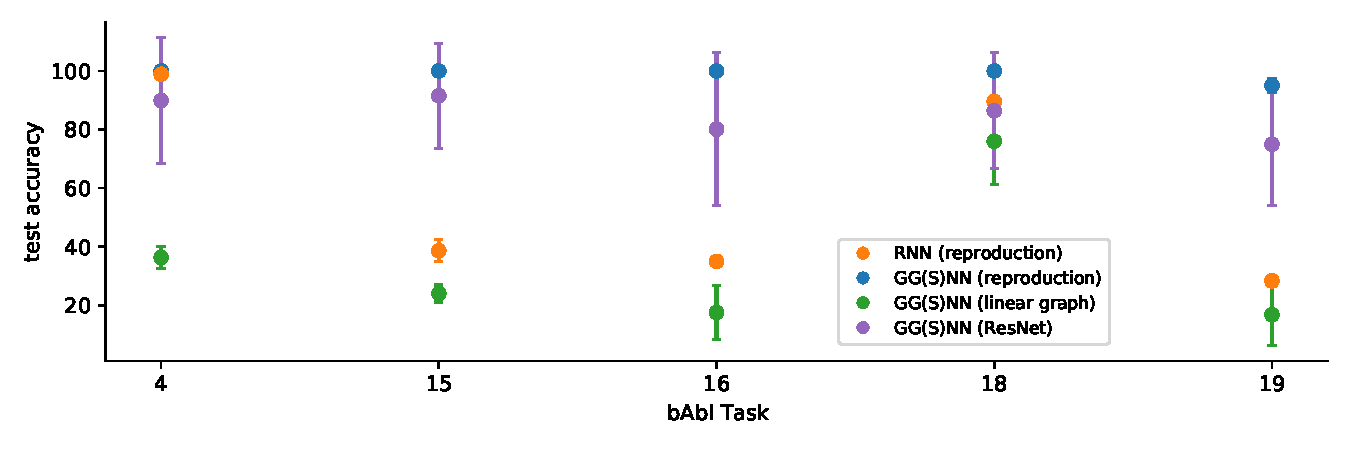
\includegraphics[width=\textwidth]{imgs/extension_plot.pdf}
            \caption{Results of the extension experiments. The drop in GGNN performance for linear graphs indicates poorer inductive bias, and increased variance of ResNets suggests better stability of GRUs.}
            \label{fig:extension}
          \end{figure}

      \textcolor{darkred}{Application: heap checking.}

      \textit{Experiment summary.}
      \vspace{0.2in}

      \textit{Findings.}
    
    \end{block}

    \begin{block}{Conclusion}
      
    \end{block}


    \begin{block}{References}
    %   \nocite{*} % Insert publications even if they are not cited in the poster
      \linespread{0.928}\selectfont
      \tiny{\printbibliography}
    \end{block}
    
    

  \end{column} % End of the 3rd column

  \begin{column}{.02\textwidth}\end{column} % Empty spacer column

\end{columns} % End of all the columns in the poster

\end{frame} % End of the enclosing frame

\end{document}